\documentclass[11pt,a4paper]{article}

\usepackage[margin=2.4cm,top=2.2cm,bottom=2.4cm]{geometry}
\usepackage{mathpazo}
\usepackage[T1]{fontenc}
\usepackage[utf8]{inputenc}
\usepackage{amsmath,amssymb}
\usepackage{booktabs}
\usepackage{xcolor}
\usepackage{tikz}
\usepackage{titlesec}
\usepackage{enumitem}
\usepackage{array}
\usepackage[hidelinks]{hyperref}
\usetikzlibrary{arrows.meta,positioning,calc}

\definecolor{ink}{HTML}{16211E}
\definecolor{pine}{HTML}{1E5B4F}
\definecolor{mulberry}{HTML}{8C3A56}
\definecolor{slate}{HTML}{54655F}
\definecolor{rulec}{HTML}{C6D2CD}
\definecolor{boxbg}{HTML}{F4F7F6}

\color{ink}

\titleformat{\section}{\large\bfseries\color{pine}}{\thesection.}{0.6em}{}
\titlespacing*{\section}{0pt}{1.6em}{0.6em}
\titleformat{\subsection}[runin]{\bfseries}{}{0em}{}[\;---]
\titlespacing*{\subsection}{0pt}{0.7em}{0.4em}

\newcommand{\stephead}[2]{%
  \vspace{1.1em}\noindent
  {\color{slate}\ttfamily\footnotesize STEP #1}\\[-0.15em]
  {\large\bfseries\color{pine} #2}\\[0.25em]
  {\color{rulec}\rule{\linewidth}{0.6pt}}\\[0.3em]}

\newcommand{\field}[1]{\smallskip\noindent\textbf{#1}\ }
\newcommand{\code}[1]{\texttt{\small #1}}

\setlength{\parindent}{0pt}
\setlength{\parskip}{0.45em}

\begin{document}

\begin{center}
  {\color{slate}\ttfamily\footnotesize IJF $\cdot$ LINK DISCOVERY $\cdot$ FAVOURITISM (FAV 13)}\\[0.5em]
  {\LARGE\bfseries Procurement Favouritism: Pipeline Specification}\\[0.6em]
  {\color{slate}\small What each stage computes, why it is computed that way,
   and what it tells us.}\\[0.3em]
  {\color{slate}\footnotesize 1{,}497{,}648 contracts scored against 245{,}462 lobbying registrations}
\end{center}

\vspace{0.6em}

%--------------------------------------------------------------------
\section*{What we are looking for}
\addcontentsline{toc}{section}{What we are looking for}

A company lobbies a government department. Soon after, \emph{that same department}
awards it a contract, often without competition. We rank contracts by how much they
look like this, so a reporter checks the most promising first.

The output is a \textbf{lead to verify}, never an assertion of wrongdoing.

The scoring unit is \textbf{one contract}. Scoring whole companies fails: Accenture's
single questionable contract out of 356 is averaged away to a non-competitive share of
$0.214$, and the known cases sink to the bottom half of the ranking.

%--------------------------------------------------------------------
\section*{Pipeline at a glance}

\begin{center}
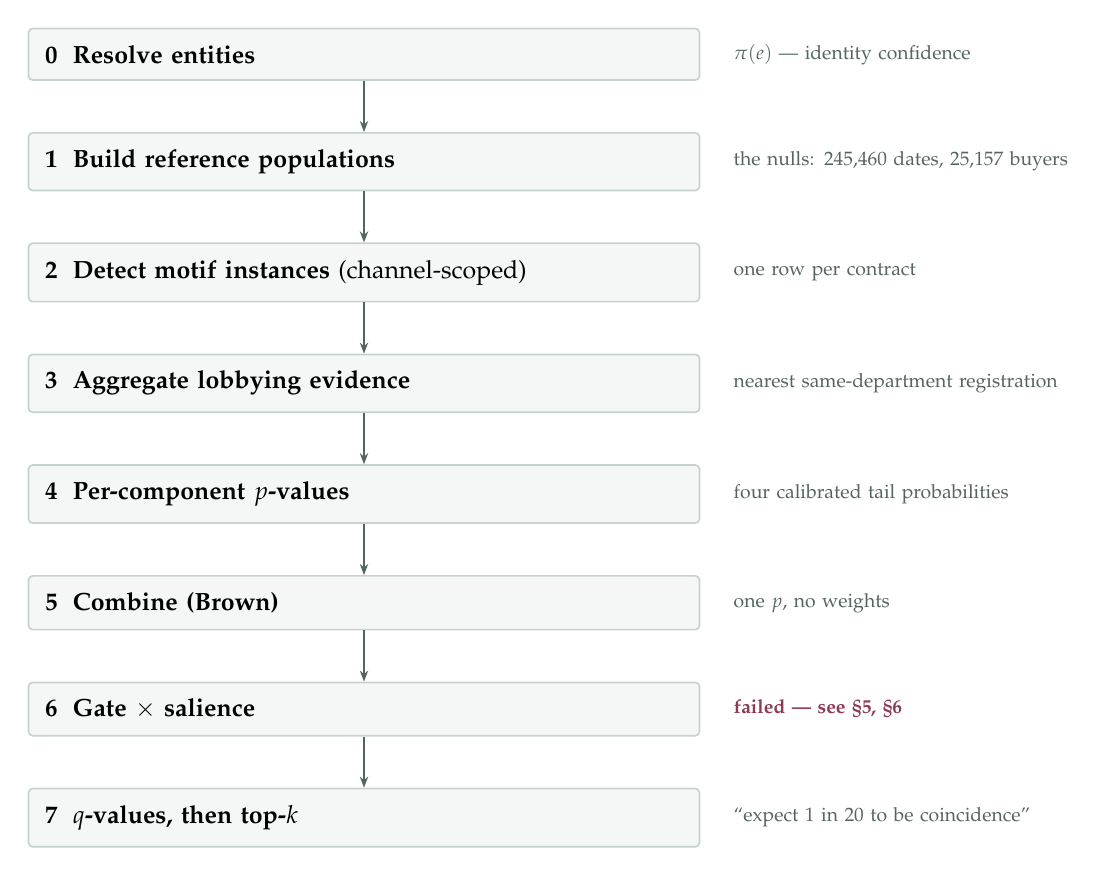
\begin{tikzpicture}[
  node distance=6.5mm,
  box/.style={draw=rulec, fill=boxbg, rounded corners=1.5pt, line width=0.6pt,
              text width=8.1cm, inner sep=6pt, align=left, font=\small},
  lbl/.style={font=\scriptsize\ttfamily, color=slate},
  ann/.style={font=\scriptsize, color=slate, text width=4.3cm, align=left},
  ar/.style={-{Stealth[length=4pt]}, draw=slate, line width=0.6pt}
]
\node[box] (s0) {\textbf{0\; Resolve entities}};
\node[box, below=of s0] (s1) {\textbf{1\; Build reference populations}};
\node[box, below=of s1] (s2) {\textbf{2\; Detect motif instances} (channel-scoped)};
\node[box, below=of s2] (s3) {\textbf{3\; Aggregate lobbying evidence}};
\node[box, below=of s3] (s4) {\textbf{4\; Per-component $p$-values}};
\node[box, below=of s4] (s5) {\textbf{5\; Combine (Brown)}};
\node[box, below=of s5] (s6) {\textbf{6\; Gate $\times$ salience}};
\node[box, below=of s6] (s7) {\textbf{7\; $q$-values, then top-$k$}};

\foreach \a/\b in {s0/s1, s1/s2, s2/s3, s3/s4, s4/s5, s5/s6, s6/s7}
  \draw[ar] (\a) -- (\b);

\node[ann, right=3mm of s0] {$\pi(e)$ --- identity confidence};
\node[ann, right=3mm of s1] {the nulls: 245{,}460 dates, 25{,}157 buyers};
\node[ann, right=3mm of s2] {one row per contract};
\node[ann, right=3mm of s3] {nearest same-department registration};
\node[ann, right=3mm of s4] {four calibrated tail probabilities};
\node[ann, right=3mm of s5] {one $p$, no weights};
\node[ann, right=3mm of s6] {\textcolor{mulberry}{\textbf{failed --- see \S5, \S6}}};
\node[ann, right=3mm of s7] {``expect 1 in 20 to be coincidence''};
\end{tikzpicture}
\end{center}

%--------------------------------------------------------------------
\section*{Notation}

\begin{center}\small
\begin{tabular}{@{}ll@{}}
\toprule
$a$ & a contract (award); $t_a$ its award date \\
$e$ & a supplier entity (one company, after name resolution) \\
$b$ & a government department (buyer) \\
$B(a)$ & the departments attached to contract $a$ \\
$\mathcal{C}_{e,b}$ & the \emph{channel}: dates on which $e$ registered to lobby $b$ \\
$R$ & the national pool of all valid lobbying start dates, $|R|=245{,}460$ \\
$n_b$ & contracts awarded by department $b$ \\
$k_b$ & of those, how many were non-competitive \\
\bottomrule
\end{tabular}
\end{center}

%====================================================================
\stephead{0}{Resolve entities, and build the identity gate}

\field{What happens.}
Raw supplier and lobbying-client names collapse into entities using the manual clusters,
then split back apart to \emph{legal} entity level.

\field{Computed.}
\[
\pi(e) \;=\; \beta(e)\cdot\Bigl(0.6 + 0.4\cdot\tfrac{\min(n_{\mathrm{reg}},\,5)}{5}\Bigr),
\qquad
\beta(e)=\begin{cases}
1.0 & \text{single name; no merge decision was ever made}\\
0.8 & \text{a manual cluster kept whole}\\
0.6 & \text{a cluster split apart on string evidence}
\end{cases}
\]

\field{Why this way.}
$\pi$ enters the final score \textbf{multiplicatively}, not additively. If
``Accenture Ltd'' is not truly the same company as ``Accenture'', there is no case at
all --- so a strong timing signal must not be able to rescue a doubtful identity. The
second factor shrinks confidence for entities resting on very few records.

Corporate families are kept \emph{separate} rather than merged: merging a parent with a
subsidiary manufactures loops (parent lobbies, subsidiary wins), and a manufactured loop
is a fabricated accusation. This costs about 11\% of identity edges.

\field{What it tells.} How much to trust that these records describe one company.
Range $0.36$ to $1.0$.

%====================================================================
\stephead{1}{Build the reference populations}

\field{What happens.} Before anything is scored, we compute what ``normal'' looks like.
Nothing is ranked at this stage.

\begin{center}\small
\begin{tabular}{@{}lll@{}}
\toprule
\textbf{Reference} & \textbf{Definition} & \textbf{Measured} \\
\midrule
$R$ & every valid national lobbying start date & 245{,}460 dates \\
$n_b,\;k_b$ & awards / non-competitive awards per department & 25{,}157 buyers \\
$\bar{g}$ & global non-competitive rate & $0.226$ \\
$W$ & all tender window lengths, sorted & 267{,}382 \\
$N_{b,e}$ & contracts from department $b$ to supplier $e$ & --- \\
$m_b$ & distinct suppliers used by $b$ & --- \\
\bottomrule
\end{tabular}
\end{center}

\field{Why this way.}
Every later $p$-value needs a denominator. ``Unusual'' is meaningless without stating
\emph{unusual compared to what}. Each reference is a population a reader can check.

\field{What it tells.} Nothing yet. It is the yardstick.

%====================================================================
\stephead{2}{Detect motif instances --- channel-scoped}

\field{What happens.}
One row per contract. For contract $a$ with supplier $e$ and departments $B(a)$, look
for prior registrations in which $e$ lobbied \emph{a department in $B(a)$}.

\field{Computed.}
\[
g \;=\; \min_{b\,\in\,B(a)}\;\Bigl(t_a - \max\{\,d \in \mathcal{C}_{e,b} : d < t_a \,\}\Bigr),
\qquad
n_{\mathrm{ch}} \;=\; \sum_{b\,\in\,B(a)} \bigl|\mathcal{C}_{e,b}\bigr|
\]

\field{Why this way.}
This is the correctness fix over the first version, which asked only \emph{``did this
supplier lobby anyone before this award?''} Under that rule, Accenture lobbying Health
Canada counted as evidence for an Accenture Defence contract. That is not a story; it is
two unrelated activities by a busy company, and the larger the company the more such
false pairings it accumulates --- reintroducing exactly the volume bias the null model
exists to remove.

\field{What it tells.}
Whether a \emph{channel} exists: a lobbying relationship with the department that
actually bought. Result: 1{,}497{,}648 instances.

%====================================================================
\stephead{3--4}{Turn each signal into a $p$-value against its own null}

Each feature becomes a genuine tail probability rather than a percentile rank. A
percentile says ``higher than 80\% of others''. A $p$-value says ``this happens 2\% of
the time'' --- a sentence a reporter can print.

\subsection*{$p_{\mathrm{time}}$: was the lobbying suspiciously recent?}
\[
Q(g) \;=\; \frac{\bigl|\{\, r \in R : t_a - g \le r < t_a \,\}\bigr|}{|R|},
\qquad
p_{\mathrm{time}} \;=\; 1-\bigl(1-Q(g)\bigr)^{\,n_{\mathrm{ch}}}
\]

\field{Why.}
Under the null, each of the $n_{\mathrm{ch}}$ registrations is placed independently at a
date drawn from the national pattern of lobbying activity. The chance that
\emph{at least one} lands within $g$ days before the award is $1-(1-Q)^n$.

\field{Improvement over v1.}
The first version required a fixed 90-day window as a free parameter, so a 3-day gap and
an 89-day gap scored identically. Using the \emph{observed} gap removes the parameter
entirely.

\field{What it tells.} How unlikely this closeness is if lobbying dates were unrelated
to award dates.

\subsection*{$p_{\mathrm{comp}}$: is sole-sourcing unusual \emph{for this department}?}
\[
\rho_b \;=\; \frac{k_b + 5\bar{g}}{n_b + 5},
\qquad
p_{\mathrm{comp}} \;=\;
\begin{cases}
\min_{b \in B(a)} \rho_b & \text{if the method is \code{NON}, \code{LIMITED} or \code{ADVANCE}}\\[2pt]
1 & \text{otherwise}
\end{cases}
\]

\field{Why.}
Departments differ. One that sole-sources 80\% of the time says nothing when it does so
again; one that sole-sources 2\% of the time is saying something. The
$5\bar{g}$ smoothing prevents a department with three contracts from producing a
spurious $0$.

\field{What it tells.} How out of character this procurement method is for this buyer.

\subsection*{$p_{\mathrm{proc}}$: was the tender open unusually briefly?}
\[
p_{\mathrm{proc}} \;=\; \widehat{F}_W(w) \;=\; \frac{\bigl|\{\,w' \in W : w' \le w \,\}\bigr|}{|W|}
\]

\field{Why.}
A wired tender is often left open just long enough to satisfy the rule. This is the
empirical distribution function --- no assumed shape.

\field{What it tells.} Whether bidders realistically had time to respond.

\subsection*{$p_{\mathrm{conc}}$: does this supplier dominate the department's book?}
\[
p_{\mathrm{conc}} \;=\; \Pr\bigl[X \ge N_{b,e}\bigr],
\qquad X \sim \mathrm{Binomial}\!\left(n_b,\ \tfrac{1}{m_b}\right)
\]

\field{Why.}
The null is ``the department spreads its awards evenly across the suppliers it uses'', so
the expected share is $n_b/m_b$. Receiving far more than that from one supplier is the
dependency signal.

\field{What it tells.} Whether this is a normal supplier relationship or a captured one.

%====================================================================
\stephead{5}{Combine, accounting for correlation}

\field{Computed.}
\[
Y_i = -2\ln p_i, \qquad X = \sum_{i=1}^{k} Y_i
\]
Under independence $X \sim \chi^2_{2k}$. Because the components are \emph{not}
independent, Brown's rescaling is applied:
\[
E = 2k, \qquad
V = \sum_{i}\sum_{j}\operatorname{cov}(Y_i, Y_j), \qquad
c = \frac{V}{2E}, \qquad
f = \frac{2E^2}{V},
\qquad
p_{\mathrm{comb}} = \Pr\!\left[\chi^2_f > \tfrac{X}{c}\right]
\]

\field{Why this way.}
Fisher's method assumes independent $p$-values. Ours are correlated --- sole-sourcing
with concentration, timing with concentration. Brown (1975) rescales the null using the
observed covariance. Crucially, \textbf{there are no weights to justify}: the dependence
structure replaces them.

\field{\textcolor{mulberry}{What actually happened --- this step broke.}}
The fit returned $c = 31.67$ and $f = 0.25$, where independence would give $c = 1$,
$f = 8$.

The cause is structural. Most contracts have \emph{no signal at all} on most components:
no lobbying gives $p_{\mathrm{time}} = 1$, a competitive award gives
$p_{\mathrm{comp}} = 1$, no tender record gives $p_{\mathrm{proc}} = 1$ --- and
$-2\ln 1 = 0$. The distribution of $X$ is therefore a large point mass at zero with a
thin tail; the variance is set entirely by outliers, inflating $c$ and collapsing $f$ to
a quarter of a degree of freedom. \textbf{Brown's method assumes roughly continuous
components; ours are mostly exact ones.} At $f = 0.25$ the output is not a calibrated
probability.

%====================================================================
\stephead{6}{Gate and salience}

\field{Computed.}
\[
\mathrm{sal}(a) = 0.5 + 0.5\cdot\min\!\left(\frac{\log(1+n^{\mathrm{aw}}_e)}{\log(1+20000)} + 0.15\,\mathbb{1}[\text{named}],\ 1\right),
\qquad
S(a) = \pi(e)\cdot\bigl(1-p_{\mathrm{comb}}\bigr)\cdot \mathrm{sal}(a)
\]

\field{Why this way.}
$\pi$ gates. Salience sits on its own axis deliberately: prominence is not
\emph{anomalous}, it is \emph{important}. The null strips volume out of the anomaly term,
while the stated objective is newsworthiness --- and newsworthy cases are prominent. Rather
than have the two fight, ``is this unusual?'' and ``would anyone care?'' are kept separate
and multiplied.

\field{\textcolor{mulberry}{What actually happened --- this hurt.}}
The full score reached AUC $0.787$ against $0.852$ for surprise alone. Once
$p_{\mathrm{comb}}$ saturated at step 5, salience --- which spans only $0.5$ to $1.0$ and
is essentially a log-compressed award count --- became the dominant discriminator. The
effect was to rebuild the prominence baseline and multiply it back in.

%====================================================================
\stephead{7}{$q$-values, then top-$k$}

\field{Computed.} Benjamini--Hochberg over the combined $p$-values:
\[
q_{(i)} \;=\; \min_{j \ge i}\ \frac{n}{j}\, p_{(j)}
\]

\field{Why this way.}
It replaces an arbitrary cut-off with a statement: \emph{``in the top 20, expect about one
to be coincidence.''} A bare score of $0.818$ tells a reporter nothing; an expected
false-positive count tells them how much checking to budget.

%====================================================================
\section*{Results}

Five companies from the 32 published favouritism stories appear in our data. We ask where
the ranking places them. No model is trained --- with five positives and no labelled
negatives there is nothing to train on. The Mann--Whitney statistic over those ranks
\emph{is} the AUC.

\begin{center}\small
\begin{tabular}{@{}lccc@{}}
\toprule
\textbf{Ranking method} & \textbf{AUC} & \textbf{Median position} & \textbf{In top 1\%} \\
\midrule
Simple rule: non-competitive, then recency & \textbf{0.983} & 0.39\% & \textbf{4 of 5} \\
Nearest lobbying gap, no null model        & 0.911 & 0.19\% & 3 of 5 \\
This pipeline, surprise only               & 0.852 & 3.04\% & 2 of 5 \\
\textcolor{mulberry}{This pipeline, full score} & \textcolor{mulberry}{0.787} & \textcolor{mulberry}{19.31\%} & \textcolor{mulberry}{0 of 5} \\
Company size only (prominence)             & 0.541 & 39.55\% & 0 of 5 \\
\bottomrule
\end{tabular}
\end{center}

Accenture's best contract ranks \textbf{76th} of 1{,}497{,}648 under the simple rule and
\textbf{77{,}255th} under the full pipeline.

\subsection*{The caveat that outweighs the table}

With five positives, an AUC estimate carries roughly $\pm 0.15$ of uncertainty. The top
three methods ($0.983$, $0.911$, $0.852$) are \textbf{statistically indistinguishable}.
The only defensible claim is that \emph{something} beats company size.

We therefore cannot select a scoring function with the evidence currently available. The
binding constraint is the ground truth, not the algorithm: further tuning would be
fitting to five points.

%====================================================================
\section*{Summary of what works and what does not}

\begin{center}\small
\begin{tabular}{@{}llp{7.4cm}@{}}
\toprule
\textbf{Stage} & \textbf{Status} & \textbf{Note} \\
\midrule
0 Identity gate        & sound & multiplicative, interpretable, four-level ladder \\
1 Reference populations& sound & each null is a stated, checkable population \\
2 Channel scoping      & sound & the main correctness fix over v1 \\
3--4 Component $p$-values & sound & surprise alone reaches AUC $0.852$; Accenture at rank 236 \\
5 Brown combination    & \textcolor{mulberry}{broken} & degenerates on components with a point mass at $p=1$ \\
6 Salience             & \textcolor{mulberry}{harmful} & $-0.065$ AUC; reintroduces the prominence confound \\
7 $q$-values           & sound & but only as meaningful as step 5 \\
\bottomrule
\end{tabular}
\end{center}

The two-line baseline that outperformed everything is, in effect, steps 2 and 4 with no
combination layer at all. The signal in this data is concentrated in two variables, and
the aggregation machinery placed on top of them subtracted value rather than adding it.

\subsection*{Repairs, in order of value}

\begin{enumerate}[leftmargin=1.4em,itemsep=0.25em]
\item \textbf{Expand and verify the ground truth.} Nothing else moves the needle. The 32
      story records were extracted automatically and none has been checked by a person.
\item \textbf{Obtain contract values.} Absent from the corpus. A \$210M no-bid contract
      and a \$5{,}000 one are currently indistinguishable to the scorer.
\item \textbf{Repair or replace step 5.} Combine only over components that actually
      fired, or model the point mass at $p=1$ explicitly. A simpler alternative is to rank
      by the minimum $p$-value with a \v{S}id\'ak correction for the number of testable
      components.
\item \textbf{Remove salience from the product.} If prominence belongs in the output it
      should be a separately reported axis, not a multiplier.
\end{enumerate}

\end{document}
